% !TEX program = tectonic
\documentclass[10pt,a4paper,twocolumn]{article}
\usepackage[margin=1.05cm]{geometry}
\usepackage[T1]{fontenc}
\usepackage[utf8]{inputenc}
\usepackage{lmodern}
\usepackage[french]{babel}
\usepackage{amsmath,amssymb}
\usepackage{booktabs,array,tabularx}
\usepackage{enumitem}
\usepackage{microtype}
\usepackage{xcolor}
\usepackage{graphicx}
\usepackage{titlesec}
\definecolor{bleu}{RGB}{20,45,90}
\definecolor{gris}{RGB}{90,90,90}
\definecolor{vert}{RGB}{20,110,60}
\definecolor{rouge}{RGB}{160,30,30}
\definecolor{orange}{RGB}{196,123,0}
\setlength{\columnsep}{0.55cm}
\raggedbottom
\setlength{\parindent}{0pt}
\setlength{\parskip}{2pt}
\setlist[itemize]{leftmargin=*,topsep=1pt,itemsep=0.5pt,parsep=0pt}
\titleformat{\section}{\normalsize\bfseries\color{bleu}}{}{0pt}{}[\vspace{-3pt}\titlerule]
\titlespacing*{\section}{0pt}{5pt}{2pt}
\begin{document}

\twocolumn[{\centering
{\LARGE\bfseries FICHE --- Notebook 10 $\cdot$ le stock des divulgations\par}
\vspace{2pt}
{\small ce que fait \texttt{10\_Stock\_Divulgations\_MathSpec.ipynb} (34 cellules, branche \texttt{v1-house}, \texttt{01\_v1\_house/}) --- tout est exécuté et vérifié $\cdot$ \textbf{aucun résultat E1/E2 encore calculé} (\S5 verrouillé)\par}
\vspace{6pt}
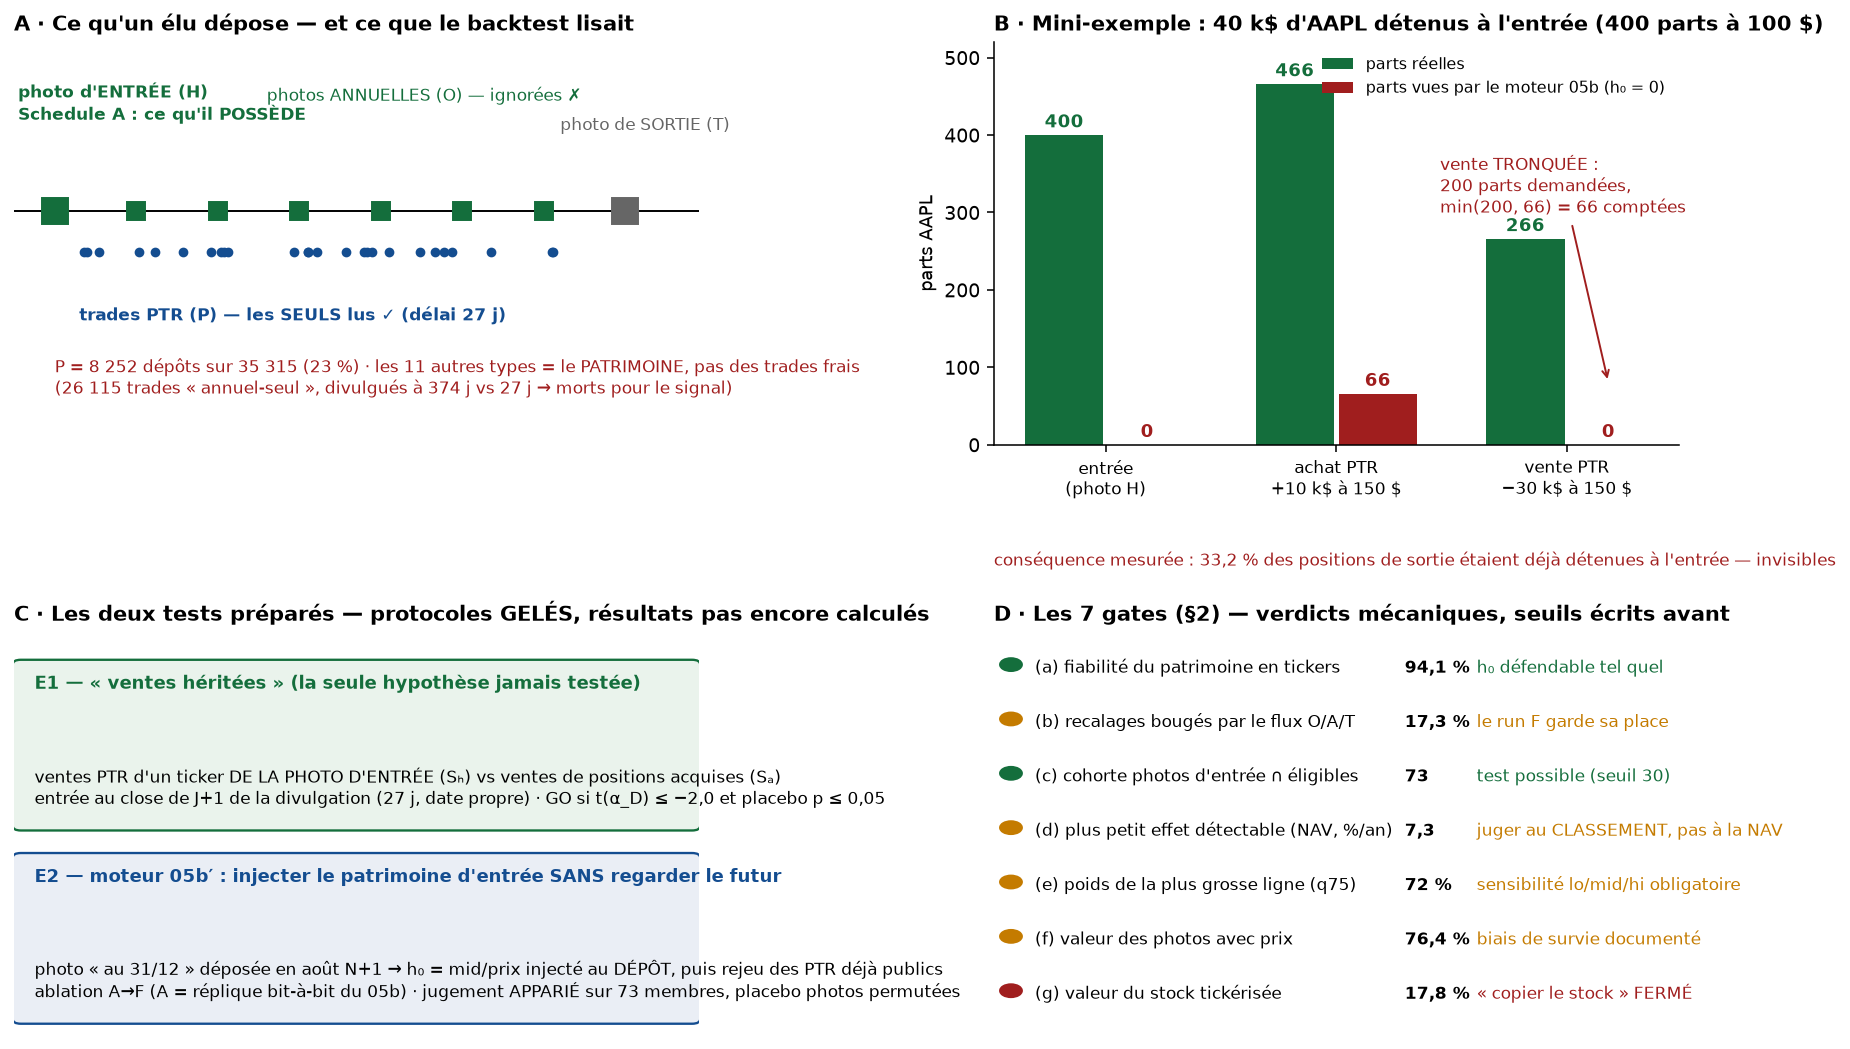
\includegraphics[width=\textwidth]{figures/fig_10_explication.png}
\vspace{2pt}}]

\section{Le problème, en 4 chiffres}
\begin{itemize}
\item le backtest lit \textbf{1 type de dépôt sur 12} : P $= 8\,252$ dépôts sur $35\,315$ (23\,\%) ;
\item le flux des 11 autres types est \textbf{mort pour le signal} : $26\,115$ trades \og{}annuel-seul\fg{}, divulgués à \textbf{374 j} (PTR : 27 j) ;
\item ce qu'ils apportent, c'est le \textbf{stock} : $420\,916$ lignes de patrimoine (Schedule A), \textbf{284} portefeuilles d'entrée datés ;
\item le moteur 05b part de $h_0=0$ : \textbf{33,2\,\%} des positions de sortie (déjà détenues à l'entrée) sont invisibles, les ventes sont tronquées ($h \leftarrow h - \min(q,h)$, panneau B).
\end{itemize}

\section{Ce que fait le notebook --- 5 blocs}
\begin{center}\small
\begin{tabularx}{\linewidth}{@{}lX@{}}
\toprule
\S0 & charge et \textbf{prouve} les données : 10 tables v1-house, sha256 $=$ MANIFEST $\cdot$ 0 orphelin de clé membre $\cdot$ fourchettes clean$\leftrightarrow$v1 : écart 0 \\
\S1 & \textbf{recopie le moteur 05b} verbatim (pattern du 07) : oracles $118\,029$ / $3\,289$ / $266$ / $223$ reproduits, 0 téléchargement \\
\S2 & mesure \textbf{7 gates} --- seuils écrits AVANT, verdicts mécaniques (panneau D) \\
\S3--\S4 & \textbf{GÈLE} les protocoles E1 et E2 --- définitions, placebos, critères GO/NO-GO \\
\S5 & \textbf{verrouillé} : s'ouvre après ta validation des gels (point d'arrêt \no2) \\
\bottomrule
\end{tabularx}
\end{center}

\section{Les 7 gates : question posée $\to$ verdict}
\begin{center}\small
\begin{tabularx}{\linewidth}{@{}Xrl@{}}
\toprule
question & mesure & verdict \\
\midrule
(a) le patrimoine en \emph{tickers} est-il fiable photo$\to$photo ? & \textbf{94,1\,\%} & \textcolor{vert}{$h_0$ défendable tel quel} \\
\quad {\scriptsize\color{gris}(vs 66,7\,\% toutes clés : le tiers d'incohérence $=$ clés-nom)} & & \\
(b) le flux O/A/T change-t-il des recalages ? & \textbf{17,3\,\%} & \textcolor{orange}{run F conservé} \\
(c) combien de membres testables ? & \textbf{73} & \textcolor{vert}{$\geq$ seuil 30} \\
(d) plus petit effet détectable sur la NAV & \textbf{7,3\,\%/an} & \textcolor{orange}{juger au classement} \\
(e) poids de la plus grosse ligne d'entrée (q75) & \textbf{72\,\%} & \textcolor{orange}{sensibilité lo/mid/hi} \\
(f) valeur des photos couverte par un prix & \textbf{76,4\,\%} & \textcolor{orange}{biais de survie documenté} \\
(g) valeur du stock tickérisée & \textbf{17,8\,\%} & \textcolor{rouge}{\og{}copier le stock\fg{} FERMÉ} \\
\bottomrule
\end{tabularx}
\end{center}
Fermetures actées avec preuve : copier le stock agrégé (g) $\cdot$ flux annuel-seul en événements (374 j $+$ placebo P1 du 08, $p=0{,}605$).

\section{E1 --- \og{}ventes héritées\fg{} (gelé)}
\begin{itemize}
\item $\Phi_0(m)$ $=$ tickers de la photo d'entrée de $m$ ; $S_h$ $=$ ventes PTR d'un ticker $\in \Phi_0(m)$, $S_a$ $=$ ventes de positions acquises en mandat ;
\item entrée au close de $J{+}1$ de la \textbf{divulgation} (27 j, date propre) ; fenêtre 252 séances ;
\item test : $D(t) = R_h(t) - R_a(t)$, $\alpha_D$ sur Carhart-4 (Newey--West) ;
\item \textbf{GO} si $t(\alpha_D) \le -2{,}0$ \textbf{et} placebo $p \le 0{,}05$ (1\,000 permutations au niveau membre) ; TOST : IC 90\,\% $\subset \pm 2\,\%$/an $\Rightarrow$ porte fermée avec borne.
\end{itemize}

\section{E2 --- moteur 05b$'$ (gelé)}
\begin{center}\small
\begin{tabularx}{\linewidth}{@{}lX@{}}
\toprule
A & témoin $\equiv$ 05b, \textbf{bit-à-bit} (266 NAV) \\
B & dates de divulgation (mesure le look-ahead du 05b) \\
C & B $+$ $h_0 = \text{mid}/P$ injecté au DÉPÔT de la photo \\
D & C $+$ recalages aux photos annuelles (audit) \\
E & D $+$ fenêtres de mandat \\
F & E $+$ flux O/A/T net (ouvert par le gate (b)) \\
\bottomrule
\end{tabularx}
\end{center}
\begin{itemize}
\item anti-look-ahead : photo \og{}au 31/12\fg{} déposée en août $N{+}1$ $\to$ injectée \textbf{au dépôt}, puis rejeu des PTR déjà publics entre les deux ;
\item jugement : \textbf{$\Delta$IC apparié} sur les 73 (bootstrap 2\,000), placebo \textbf{photos permutées} entre membres (200), sensibilité $h_0 \in \{$lo, mid, hi$\}$ ;
\item interdit : tout top-$K$ mixte (73 initialisés $+$ 150 autres) --- artefact de disponibilité.
\end{itemize}

\section{Garanties}
\begin{itemize}
\item \textbf{rien d'existant modifié} : git $=$ ajouts seulement ; \texttt{prices\_v2} snapshoté au début, re-asserté à la fin (3\,351 fichiers, intact) ;
\item cache prix \textbf{séparé} \texttt{prices\_holdings\_v1} (1\,907 séries, 2\,154 échecs consignés) --- toucher \texttt{prices\_v2} casserait les oracles du 05b/07/09 ;
\item chaque section a sa Validation (asserts bloquants) ; 1 photo d'entrée perdue, journalisée (doc \texttt{10041638}).
\end{itemize}

\section{La suite (te concerne)}
\begin{itemize}
\item \textbf{point d'arrêt \no2} : tu valides (ou amendes) les gels \S3/\S4 $\to$ j'ouvre les sections résultats ;
\item valeur attendue, dit honnêtement : E1 $=$ le seul test \emph{neuf} (un nul fermerait une vraie porte) ; E2 $=$ blindage du verdict zéro-alpha --- ou son renversement.
\end{itemize}

\end{document}
